% Created by tikzDevice version 0.7.0 on 2014-07-26 02:55:38
% !TEX encoding = UTF-8 Unicode
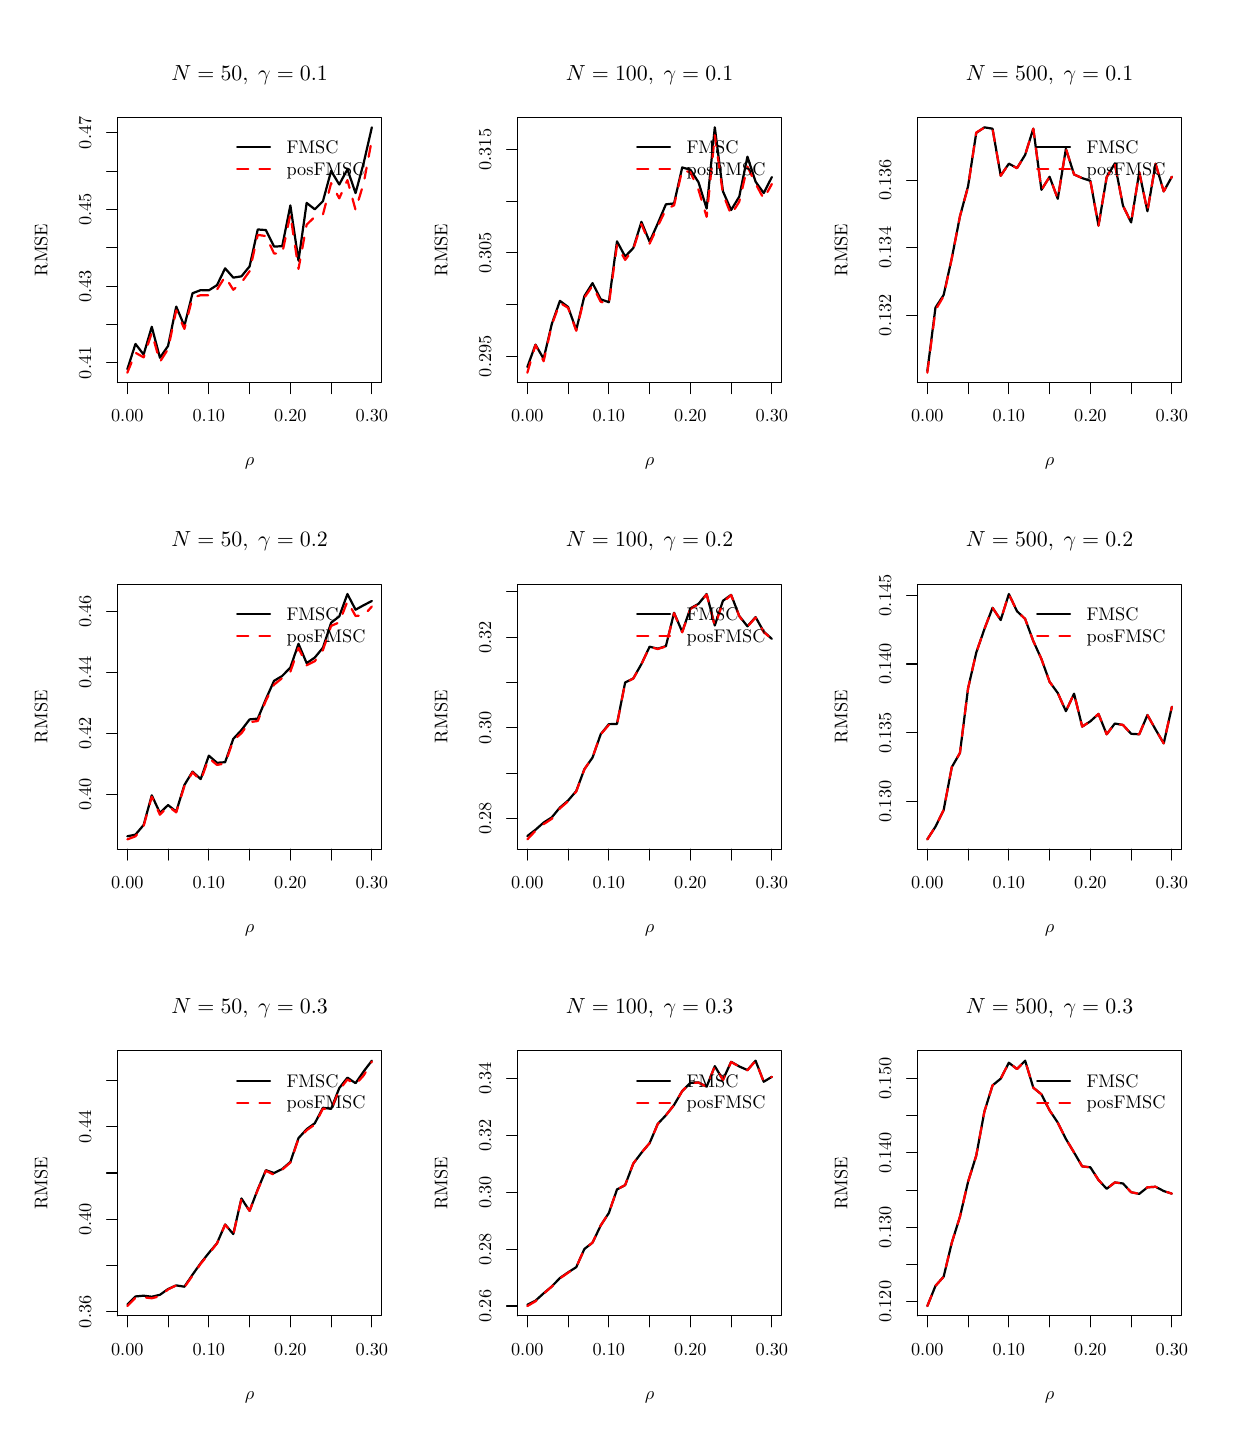
\begin{tikzpicture}[x=1pt,y=1pt]
\definecolor[named]{fillColor}{rgb}{1.00,1.00,1.00}
\path[use as bounding box,fill=fillColor,fill opacity=0.00] (0,0) rectangle (433.62,505.89);
\begin{scope}
\path[clip] ( 32.47,377.65) rectangle (127.91,473.42);
\definecolor[named]{drawColor}{rgb}{0.00,0.00,0.00}

\path[draw=drawColor,line width= 0.8pt,line join=round,line cap=round] ( 36.01,382.45) --
	( 38.95,391.60) --
	( 41.90,387.78) --
	( 44.84,397.80) --
	( 47.79,386.61) --
	( 50.73,390.88) --
	( 53.68,405.10) --
	( 56.63,398.09) --
	( 59.57,409.92) --
	( 62.52,411.05) --
	( 65.46,410.97) --
	( 68.41,412.85) --
	( 71.35,418.92) --
	( 74.30,415.57) --
	( 77.24,416.03) --
	( 80.19,419.62) --
	( 83.14,432.97) --
	( 86.08,432.75) --
	( 89.03,426.79) --
	( 91.97,426.92) --
	( 94.92,441.67) --
	( 97.86,421.70) --
	(100.81,442.56) --
	(103.75,440.25) --
	(106.70,443.21) --
	(109.65,454.12) --
	(112.59,449.21) --
	(115.54,454.71) --
	(118.48,446.10) --
	(121.43,457.07) --
	(124.37,469.87);
\end{scope}
\begin{scope}
\path[clip] (  0.00,  0.00) rectangle (433.62,505.89);
\definecolor[named]{drawColor}{rgb}{0.00,0.00,0.00}

\path[draw=drawColor,line width= 0.4pt,line join=round,line cap=round] ( 36.01,377.65) -- (124.37,377.65);

\path[draw=drawColor,line width= 0.4pt,line join=round,line cap=round] ( 36.01,377.65) -- ( 36.01,373.69);

\path[draw=drawColor,line width= 0.4pt,line join=round,line cap=round] ( 50.73,377.65) -- ( 50.73,373.69);

\path[draw=drawColor,line width= 0.4pt,line join=round,line cap=round] ( 65.46,377.65) -- ( 65.46,373.69);

\path[draw=drawColor,line width= 0.4pt,line join=round,line cap=round] ( 80.19,377.65) -- ( 80.19,373.69);

\path[draw=drawColor,line width= 0.4pt,line join=round,line cap=round] ( 94.92,377.65) -- ( 94.92,373.69);

\path[draw=drawColor,line width= 0.4pt,line join=round,line cap=round] (109.65,377.65) -- (109.65,373.69);

\path[draw=drawColor,line width= 0.4pt,line join=round,line cap=round] (124.37,377.65) -- (124.37,373.69);

\node[text=drawColor,anchor=base,inner sep=0pt, outer sep=0pt, scale=  0.66] at ( 36.01,363.40) {0.00};

\node[text=drawColor,anchor=base,inner sep=0pt, outer sep=0pt, scale=  0.66] at ( 65.46,363.40) {0.10};

\node[text=drawColor,anchor=base,inner sep=0pt, outer sep=0pt, scale=  0.66] at ( 94.92,363.40) {0.20};

\node[text=drawColor,anchor=base,inner sep=0pt, outer sep=0pt, scale=  0.66] at (124.37,363.40) {0.30};

\path[draw=drawColor,line width= 0.4pt,line join=round,line cap=round] ( 32.47,384.77) -- ( 32.47,467.91);

\path[draw=drawColor,line width= 0.4pt,line join=round,line cap=round] ( 32.47,384.77) -- ( 28.51,384.77);

\path[draw=drawColor,line width= 0.4pt,line join=round,line cap=round] ( 32.47,398.63) -- ( 28.51,398.63);

\path[draw=drawColor,line width= 0.4pt,line join=round,line cap=round] ( 32.47,412.48) -- ( 28.51,412.48);

\path[draw=drawColor,line width= 0.4pt,line join=round,line cap=round] ( 32.47,426.34) -- ( 28.51,426.34);

\path[draw=drawColor,line width= 0.4pt,line join=round,line cap=round] ( 32.47,440.20) -- ( 28.51,440.20);

\path[draw=drawColor,line width= 0.4pt,line join=round,line cap=round] ( 32.47,454.05) -- ( 28.51,454.05);

\path[draw=drawColor,line width= 0.4pt,line join=round,line cap=round] ( 32.47,467.91) -- ( 28.51,467.91);

\node[text=drawColor,rotate= 90.00,anchor=base,inner sep=0pt, outer sep=0pt, scale=  0.66] at ( 22.97,384.77) {0.41};

\node[text=drawColor,rotate= 90.00,anchor=base,inner sep=0pt, outer sep=0pt, scale=  0.66] at ( 22.97,412.48) {0.43};

\node[text=drawColor,rotate= 90.00,anchor=base,inner sep=0pt, outer sep=0pt, scale=  0.66] at ( 22.97,440.20) {0.45};

\node[text=drawColor,rotate= 90.00,anchor=base,inner sep=0pt, outer sep=0pt, scale=  0.66] at ( 22.97,467.91) {0.47};

\path[draw=drawColor,line width= 0.4pt,line join=round,line cap=round] ( 32.47,377.65) --
	(127.91,377.65) --
	(127.91,473.42) --
	( 32.47,473.42) --
	( 32.47,377.65);
\end{scope}
\begin{scope}
\path[clip] (  0.00,337.26) rectangle (144.54,505.89);
\definecolor[named]{drawColor}{rgb}{0.00,0.00,0.00}

\node[text=drawColor,anchor=base,inner sep=0pt, outer sep=0pt, scale=  0.79] at ( 80.19,486.92) {\bfseries $N=50, \;\gamma=0.1$};

\node[text=drawColor,anchor=base,inner sep=0pt, outer sep=0pt, scale=  0.66] at ( 80.19,347.56) {$\rho$};

\node[text=drawColor,rotate= 90.00,anchor=base,inner sep=0pt, outer sep=0pt, scale=  0.66] at (  7.13,425.53) {RMSE};
\end{scope}
\begin{scope}
\path[clip] ( 32.47,377.65) rectangle (127.91,473.42);
\definecolor[named]{drawColor}{rgb}{1.00,0.00,0.00}

\path[draw=drawColor,line width= 0.8pt,dash pattern=on 4pt off 4pt ,line join=round,line cap=round] ( 36.01,381.20) --
	( 38.95,388.42) --
	( 41.90,386.75) --
	( 44.84,395.61) --
	( 47.79,385.13) --
	( 50.73,389.77) --
	( 53.68,403.74) --
	( 56.63,397.04) --
	( 59.57,408.36) --
	( 62.52,409.22) --
	( 65.46,409.15) --
	( 68.41,411.25) --
	( 71.35,415.92) --
	( 74.30,411.16) --
	( 77.24,413.79) --
	( 80.19,417.89) --
	( 83.14,431.02) --
	( 86.08,430.57) --
	( 89.03,424.30) --
	( 91.97,424.28) --
	( 94.92,438.38) --
	( 97.86,418.72) --
	(100.81,434.71) --
	(103.75,437.54) --
	(106.70,438.39) --
	(109.65,449.71) --
	(112.59,444.22) --
	(115.54,450.79) --
	(118.48,440.05) --
	(121.43,449.77) --
	(124.37,465.42);
\definecolor[named]{drawColor}{rgb}{0.00,0.00,0.00}

\path[draw=drawColor,line width= 0.8pt,line join=round,line cap=round] ( 75.72,462.63) -- ( 87.60,462.63);
\definecolor[named]{drawColor}{rgb}{1.00,0.00,0.00}

\path[draw=drawColor,line width= 0.8pt,dash pattern=on 4pt off 4pt ,line join=round,line cap=round] ( 75.72,454.71) -- ( 87.60,454.71);
\definecolor[named]{drawColor}{rgb}{0.00,0.00,0.00}

\node[text=drawColor,anchor=base west,inner sep=0pt, outer sep=0pt, scale=  0.66] at ( 93.54,460.35) {FMSC};

\node[text=drawColor,anchor=base west,inner sep=0pt, outer sep=0pt, scale=  0.66] at ( 93.54,452.43) {posFMSC};
\end{scope}
\begin{scope}
\path[clip] (177.01,377.65) rectangle (272.45,473.42);
\definecolor[named]{drawColor}{rgb}{0.00,0.00,0.00}

\path[draw=drawColor,line width= 0.8pt,line join=round,line cap=round] (180.55,383.25) --
	(183.49,391.35) --
	(186.44,386.25) --
	(189.38,398.78) --
	(192.33,407.17) --
	(195.27,404.96) --
	(198.22,396.66) --
	(201.17,408.91) --
	(204.11,413.59) --
	(207.06,407.75) --
	(210.00,406.67) --
	(212.95,428.68) --
	(215.89,423.19) --
	(218.84,426.24) --
	(221.78,435.72) --
	(224.73,428.54) --
	(227.68,435.12) --
	(230.62,442.05) --
	(233.57,442.37) --
	(236.51,455.37) --
	(239.46,454.56) --
	(242.40,450.04) --
	(245.35,440.51) --
	(248.29,469.87) --
	(251.24,446.73) --
	(254.19,439.98) --
	(257.13,444.84) --
	(260.08,459.29) --
	(263.02,450.24) --
	(265.97,446.11) --
	(268.91,451.91);
\end{scope}
\begin{scope}
\path[clip] (  0.00,  0.00) rectangle (433.62,505.89);
\definecolor[named]{drawColor}{rgb}{0.00,0.00,0.00}

\path[draw=drawColor,line width= 0.4pt,line join=round,line cap=round] (180.55,377.65) -- (268.91,377.65);

\path[draw=drawColor,line width= 0.4pt,line join=round,line cap=round] (180.55,377.65) -- (180.55,373.69);

\path[draw=drawColor,line width= 0.4pt,line join=round,line cap=round] (195.27,377.65) -- (195.27,373.69);

\path[draw=drawColor,line width= 0.4pt,line join=round,line cap=round] (210.00,377.65) -- (210.00,373.69);

\path[draw=drawColor,line width= 0.4pt,line join=round,line cap=round] (224.73,377.65) -- (224.73,373.69);

\path[draw=drawColor,line width= 0.4pt,line join=round,line cap=round] (239.46,377.65) -- (239.46,373.69);

\path[draw=drawColor,line width= 0.4pt,line join=round,line cap=round] (254.19,377.65) -- (254.19,373.69);

\path[draw=drawColor,line width= 0.4pt,line join=round,line cap=round] (268.91,377.65) -- (268.91,373.69);

\node[text=drawColor,anchor=base,inner sep=0pt, outer sep=0pt, scale=  0.66] at (180.55,363.40) {0.00};

\node[text=drawColor,anchor=base,inner sep=0pt, outer sep=0pt, scale=  0.66] at (210.00,363.40) {0.10};

\node[text=drawColor,anchor=base,inner sep=0pt, outer sep=0pt, scale=  0.66] at (239.46,363.40) {0.20};

\node[text=drawColor,anchor=base,inner sep=0pt, outer sep=0pt, scale=  0.66] at (268.91,363.40) {0.30};

\path[draw=drawColor,line width= 0.4pt,line join=round,line cap=round] (177.01,387.17) -- (177.01,461.85);

\path[draw=drawColor,line width= 0.4pt,line join=round,line cap=round] (177.01,387.17) -- (173.05,387.17);

\path[draw=drawColor,line width= 0.4pt,line join=round,line cap=round] (177.01,405.84) -- (173.05,405.84);

\path[draw=drawColor,line width= 0.4pt,line join=round,line cap=round] (177.01,424.51) -- (173.05,424.51);

\path[draw=drawColor,line width= 0.4pt,line join=round,line cap=round] (177.01,443.18) -- (173.05,443.18);

\path[draw=drawColor,line width= 0.4pt,line join=round,line cap=round] (177.01,461.85) -- (173.05,461.85);

\node[text=drawColor,rotate= 90.00,anchor=base,inner sep=0pt, outer sep=0pt, scale=  0.66] at (167.51,387.17) {0.295};

\node[text=drawColor,rotate= 90.00,anchor=base,inner sep=0pt, outer sep=0pt, scale=  0.66] at (167.51,424.51) {0.305};

\node[text=drawColor,rotate= 90.00,anchor=base,inner sep=0pt, outer sep=0pt, scale=  0.66] at (167.51,461.85) {0.315};

\path[draw=drawColor,line width= 0.4pt,line join=round,line cap=round] (177.01,377.65) --
	(272.45,377.65) --
	(272.45,473.42) --
	(177.01,473.42) --
	(177.01,377.65);
\end{scope}
\begin{scope}
\path[clip] (144.54,337.26) rectangle (289.08,505.89);
\definecolor[named]{drawColor}{rgb}{0.00,0.00,0.00}

\node[text=drawColor,anchor=base,inner sep=0pt, outer sep=0pt, scale=  0.79] at (224.73,486.92) {\bfseries $N=100, \;\gamma=0.1$};

\node[text=drawColor,anchor=base,inner sep=0pt, outer sep=0pt, scale=  0.66] at (224.73,347.56) {$\rho$};

\node[text=drawColor,rotate= 90.00,anchor=base,inner sep=0pt, outer sep=0pt, scale=  0.66] at (151.67,425.54) {RMSE};
\end{scope}
\begin{scope}
\path[clip] (177.01,377.65) rectangle (272.45,473.42);
\definecolor[named]{drawColor}{rgb}{1.00,0.00,0.00}

\path[draw=drawColor,line width= 0.8pt,dash pattern=on 4pt off 4pt ,line join=round,line cap=round] (180.55,381.20) --
	(183.49,391.24) --
	(186.44,385.34) --
	(189.38,398.47) --
	(192.33,406.46) --
	(195.27,404.65) --
	(198.22,396.36) --
	(201.17,408.32) --
	(204.11,412.63) --
	(207.06,406.86) --
	(210.00,405.87) --
	(212.95,427.26) --
	(215.89,421.97) --
	(218.84,425.89) --
	(221.78,434.91) --
	(224.73,427.85) --
	(227.68,434.12) --
	(230.62,440.25) --
	(233.57,441.69) --
	(236.51,454.42) --
	(239.46,453.65) --
	(242.40,447.31) --
	(245.35,437.52) --
	(248.29,467.02) --
	(251.24,445.77) --
	(254.19,438.29) --
	(257.13,443.02) --
	(260.08,455.70) --
	(263.02,449.52) --
	(265.97,444.04) --
	(268.91,449.39);
\definecolor[named]{drawColor}{rgb}{0.00,0.00,0.00}

\path[draw=drawColor,line width= 0.8pt,line join=round,line cap=round] (220.26,462.63) -- (232.14,462.63);
\definecolor[named]{drawColor}{rgb}{1.00,0.00,0.00}

\path[draw=drawColor,line width= 0.8pt,dash pattern=on 4pt off 4pt ,line join=round,line cap=round] (220.26,454.71) -- (232.14,454.71);
\definecolor[named]{drawColor}{rgb}{0.00,0.00,0.00}

\node[text=drawColor,anchor=base west,inner sep=0pt, outer sep=0pt, scale=  0.66] at (238.08,460.35) {FMSC};

\node[text=drawColor,anchor=base west,inner sep=0pt, outer sep=0pt, scale=  0.66] at (238.08,452.43) {posFMSC};
\end{scope}
\begin{scope}
\path[clip] (321.55,377.65) rectangle (416.99,473.42);
\definecolor[named]{drawColor}{rgb}{0.00,0.00,0.00}

\path[draw=drawColor,line width= 0.8pt,line join=round,line cap=round] (325.09,381.80) --
	(328.03,404.74) --
	(330.98,409.28) --
	(333.92,422.56) --
	(336.87,437.67) --
	(339.81,448.61) --
	(342.76,467.86) --
	(345.71,469.87) --
	(348.65,469.38) --
	(351.60,452.39) --
	(354.54,456.75) --
	(357.49,455.14) --
	(360.43,459.92) --
	(363.38,469.41) --
	(366.32,447.28) --
	(369.27,452.01) --
	(372.22,444.06) --
	(375.16,462.13) --
	(378.11,452.85) --
	(381.05,451.53) --
	(384.00,450.55) --
	(386.94,434.33) --
	(389.89,451.88) --
	(392.83,456.79) --
	(395.78,441.56) --
	(398.73,435.51) --
	(401.67,453.71) --
	(404.62,439.56) --
	(407.56,456.71) --
	(410.51,446.71) --
	(413.45,452.03);
\end{scope}
\begin{scope}
\path[clip] (  0.00,  0.00) rectangle (433.62,505.89);
\definecolor[named]{drawColor}{rgb}{0.00,0.00,0.00}

\path[draw=drawColor,line width= 0.4pt,line join=round,line cap=round] (325.09,377.65) -- (413.45,377.65);

\path[draw=drawColor,line width= 0.4pt,line join=round,line cap=round] (325.09,377.65) -- (325.09,373.69);

\path[draw=drawColor,line width= 0.4pt,line join=round,line cap=round] (339.81,377.65) -- (339.81,373.69);

\path[draw=drawColor,line width= 0.4pt,line join=round,line cap=round] (354.54,377.65) -- (354.54,373.69);

\path[draw=drawColor,line width= 0.4pt,line join=round,line cap=round] (369.27,377.65) -- (369.27,373.69);

\path[draw=drawColor,line width= 0.4pt,line join=round,line cap=round] (384.00,377.65) -- (384.00,373.69);

\path[draw=drawColor,line width= 0.4pt,line join=round,line cap=round] (398.73,377.65) -- (398.73,373.69);

\path[draw=drawColor,line width= 0.4pt,line join=round,line cap=round] (413.45,377.65) -- (413.45,373.69);

\node[text=drawColor,anchor=base,inner sep=0pt, outer sep=0pt, scale=  0.66] at (325.09,363.40) {0.00};

\node[text=drawColor,anchor=base,inner sep=0pt, outer sep=0pt, scale=  0.66] at (354.54,363.40) {0.10};

\node[text=drawColor,anchor=base,inner sep=0pt, outer sep=0pt, scale=  0.66] at (384.00,363.40) {0.20};

\node[text=drawColor,anchor=base,inner sep=0pt, outer sep=0pt, scale=  0.66] at (413.45,363.40) {0.30};

\path[draw=drawColor,line width= 0.4pt,line join=round,line cap=round] (321.55,401.98) -- (321.55,450.82);

\path[draw=drawColor,line width= 0.4pt,line join=round,line cap=round] (321.55,401.98) -- (317.59,401.98);

\path[draw=drawColor,line width= 0.4pt,line join=round,line cap=round] (321.55,426.40) -- (317.59,426.40);

\path[draw=drawColor,line width= 0.4pt,line join=round,line cap=round] (321.55,450.82) -- (317.59,450.82);

\node[text=drawColor,rotate= 90.00,anchor=base,inner sep=0pt, outer sep=0pt, scale=  0.66] at (312.05,401.98) {0.132};

\node[text=drawColor,rotate= 90.00,anchor=base,inner sep=0pt, outer sep=0pt, scale=  0.66] at (312.05,426.40) {0.134};

\node[text=drawColor,rotate= 90.00,anchor=base,inner sep=0pt, outer sep=0pt, scale=  0.66] at (312.05,450.82) {0.136};

\path[draw=drawColor,line width= 0.4pt,line join=round,line cap=round] (321.55,377.65) --
	(416.99,377.65) --
	(416.99,473.42) --
	(321.55,473.42) --
	(321.55,377.65);
\end{scope}
\begin{scope}
\path[clip] (289.08,337.26) rectangle (433.62,505.89);
\definecolor[named]{drawColor}{rgb}{0.00,0.00,0.00}

\node[text=drawColor,anchor=base,inner sep=0pt, outer sep=0pt, scale=  0.79] at (369.27,486.92) {\bfseries $N=500, \;\gamma=0.1$};

\node[text=drawColor,anchor=base,inner sep=0pt, outer sep=0pt, scale=  0.66] at (369.27,347.56) {$\rho$};

\node[text=drawColor,rotate= 90.00,anchor=base,inner sep=0pt, outer sep=0pt, scale=  0.66] at (296.21,425.53) {RMSE};
\end{scope}
\begin{scope}
\path[clip] (321.55,377.65) rectangle (416.99,473.42);
\definecolor[named]{drawColor}{rgb}{1.00,0.00,0.00}

\path[draw=drawColor,line width= 0.8pt,dash pattern=on 4pt off 4pt ,line join=round,line cap=round] (325.09,381.20) --
	(328.03,403.84) --
	(330.98,408.85) --
	(333.92,422.46) --
	(336.87,437.72) --
	(339.81,448.34) --
	(342.76,467.99) --
	(345.71,469.77) --
	(348.65,469.35) --
	(351.60,452.37) --
	(354.54,456.74) --
	(357.49,455.10) --
	(360.43,459.88) --
	(363.38,469.39) --
	(366.32,447.27) --
	(369.27,452.00) --
	(372.22,444.06) --
	(375.16,462.12) --
	(378.11,452.85) --
	(381.05,451.53) --
	(384.00,450.55) --
	(386.94,434.33) --
	(389.89,451.88) --
	(392.83,456.79) --
	(395.78,441.56) --
	(398.73,435.51) --
	(401.67,453.71) --
	(404.62,439.56) --
	(407.56,456.71) --
	(410.51,446.71) --
	(413.45,452.03);
\definecolor[named]{drawColor}{rgb}{0.00,0.00,0.00}

\path[draw=drawColor,line width= 0.8pt,line join=round,line cap=round] (364.80,462.63) -- (376.68,462.63);
\definecolor[named]{drawColor}{rgb}{1.00,0.00,0.00}

\path[draw=drawColor,line width= 0.8pt,dash pattern=on 4pt off 4pt ,line join=round,line cap=round] (364.80,454.71) -- (376.68,454.71);
\definecolor[named]{drawColor}{rgb}{0.00,0.00,0.00}

\node[text=drawColor,anchor=base west,inner sep=0pt, outer sep=0pt, scale=  0.66] at (382.62,460.35) {FMSC};

\node[text=drawColor,anchor=base west,inner sep=0pt, outer sep=0pt, scale=  0.66] at (382.62,452.43) {posFMSC};
\end{scope}
\begin{scope}
\path[clip] ( 32.47,209.02) rectangle (127.91,304.79);
\definecolor[named]{drawColor}{rgb}{0.00,0.00,0.00}

\path[draw=drawColor,line width= 0.8pt,line join=round,line cap=round] ( 36.01,213.70) --
	( 38.95,214.29) --
	( 41.90,217.78) --
	( 44.84,228.50) --
	( 47.79,222.15) --
	( 50.73,224.98) --
	( 53.68,222.62) --
	( 56.63,232.22) --
	( 59.57,237.07) --
	( 62.52,234.36) --
	( 65.46,242.83) --
	( 68.41,240.25) --
	( 71.35,240.47) --
	( 74.30,248.90) --
	( 77.24,252.07) --
	( 80.19,255.93) --
	( 83.14,256.22) --
	( 86.08,263.27) --
	( 89.03,269.87) --
	( 91.97,271.62) --
	( 94.92,274.67) --
	( 97.86,283.25) --
	(100.81,276.25) --
	(103.75,278.27) --
	(106.70,281.86) --
	(109.65,290.88) --
	(112.59,293.14) --
	(115.54,301.24) --
	(118.48,295.57) --
	(121.43,297.20) --
	(124.37,298.72);
\end{scope}
\begin{scope}
\path[clip] (  0.00,  0.00) rectangle (433.62,505.89);
\definecolor[named]{drawColor}{rgb}{0.00,0.00,0.00}

\path[draw=drawColor,line width= 0.4pt,line join=round,line cap=round] ( 36.01,209.02) -- (124.37,209.02);

\path[draw=drawColor,line width= 0.4pt,line join=round,line cap=round] ( 36.01,209.02) -- ( 36.01,205.06);

\path[draw=drawColor,line width= 0.4pt,line join=round,line cap=round] ( 50.73,209.02) -- ( 50.73,205.06);

\path[draw=drawColor,line width= 0.4pt,line join=round,line cap=round] ( 65.46,209.02) -- ( 65.46,205.06);

\path[draw=drawColor,line width= 0.4pt,line join=round,line cap=round] ( 80.19,209.02) -- ( 80.19,205.06);

\path[draw=drawColor,line width= 0.4pt,line join=round,line cap=round] ( 94.92,209.02) -- ( 94.92,205.06);

\path[draw=drawColor,line width= 0.4pt,line join=round,line cap=round] (109.65,209.02) -- (109.65,205.06);

\path[draw=drawColor,line width= 0.4pt,line join=round,line cap=round] (124.37,209.02) -- (124.37,205.06);

\node[text=drawColor,anchor=base,inner sep=0pt, outer sep=0pt, scale=  0.66] at ( 36.01,194.77) {0.00};

\node[text=drawColor,anchor=base,inner sep=0pt, outer sep=0pt, scale=  0.66] at ( 65.46,194.77) {0.10};

\node[text=drawColor,anchor=base,inner sep=0pt, outer sep=0pt, scale=  0.66] at ( 94.92,194.77) {0.20};

\node[text=drawColor,anchor=base,inner sep=0pt, outer sep=0pt, scale=  0.66] at (124.37,194.77) {0.30};

\path[draw=drawColor,line width= 0.4pt,line join=round,line cap=round] ( 32.47,228.75) -- ( 32.47,294.86);

\path[draw=drawColor,line width= 0.4pt,line join=round,line cap=round] ( 32.47,228.75) -- ( 28.51,228.75);

\path[draw=drawColor,line width= 0.4pt,line join=round,line cap=round] ( 32.47,250.79) -- ( 28.51,250.79);

\path[draw=drawColor,line width= 0.4pt,line join=round,line cap=round] ( 32.47,272.82) -- ( 28.51,272.82);

\path[draw=drawColor,line width= 0.4pt,line join=round,line cap=round] ( 32.47,294.86) -- ( 28.51,294.86);

\node[text=drawColor,rotate= 90.00,anchor=base,inner sep=0pt, outer sep=0pt, scale=  0.66] at ( 22.97,228.75) {0.40};

\node[text=drawColor,rotate= 90.00,anchor=base,inner sep=0pt, outer sep=0pt, scale=  0.66] at ( 22.97,250.79) {0.42};

\node[text=drawColor,rotate= 90.00,anchor=base,inner sep=0pt, outer sep=0pt, scale=  0.66] at ( 22.97,272.82) {0.44};

\node[text=drawColor,rotate= 90.00,anchor=base,inner sep=0pt, outer sep=0pt, scale=  0.66] at ( 22.97,294.86) {0.46};

\path[draw=drawColor,line width= 0.4pt,line join=round,line cap=round] ( 32.47,209.02) --
	(127.91,209.02) --
	(127.91,304.79) --
	( 32.47,304.79) --
	( 32.47,209.02);
\end{scope}
\begin{scope}
\path[clip] (  0.00,168.63) rectangle (144.54,337.26);
\definecolor[named]{drawColor}{rgb}{0.00,0.00,0.00}

\node[text=drawColor,anchor=base,inner sep=0pt, outer sep=0pt, scale=  0.79] at ( 80.19,318.29) {\bfseries $N=50, \;\gamma=0.2$};

\node[text=drawColor,anchor=base,inner sep=0pt, outer sep=0pt, scale=  0.66] at ( 80.19,178.93) {$\rho$};

\node[text=drawColor,rotate= 90.00,anchor=base,inner sep=0pt, outer sep=0pt, scale=  0.66] at (  7.13,256.90) {RMSE};
\end{scope}
\begin{scope}
\path[clip] ( 32.47,209.02) rectangle (127.91,304.79);
\definecolor[named]{drawColor}{rgb}{1.00,0.00,0.00}

\path[draw=drawColor,line width= 0.8pt,dash pattern=on 4pt off 4pt ,line join=round,line cap=round] ( 36.01,212.57) --
	( 38.95,213.68) --
	( 41.90,217.41) --
	( 44.84,227.98) --
	( 47.79,221.48) --
	( 50.73,224.61) --
	( 53.68,222.34) --
	( 56.63,231.83) --
	( 59.57,236.84) --
	( 62.52,233.87) --
	( 65.46,241.91) --
	( 68.41,239.49) --
	( 71.35,240.02) --
	( 74.30,248.36) --
	( 77.24,250.95) --
	( 80.19,254.93) --
	( 83.14,255.35) --
	( 86.08,262.73) --
	( 89.03,268.49) --
	( 91.97,270.85) --
	( 94.92,273.12) --
	( 97.86,281.78) --
	(100.81,275.50) --
	(103.75,276.96) --
	(106.70,281.00) --
	(109.65,289.72) --
	(112.59,290.99) --
	(115.54,298.58) --
	(118.48,293.32) --
	(121.43,293.45) --
	(124.37,296.72);
\definecolor[named]{drawColor}{rgb}{0.00,0.00,0.00}

\path[draw=drawColor,line width= 0.8pt,line join=round,line cap=round] ( 75.72,294.00) -- ( 87.60,294.00);
\definecolor[named]{drawColor}{rgb}{1.00,0.00,0.00}

\path[draw=drawColor,line width= 0.8pt,dash pattern=on 4pt off 4pt ,line join=round,line cap=round] ( 75.72,286.08) -- ( 87.60,286.08);
\definecolor[named]{drawColor}{rgb}{0.00,0.00,0.00}

\node[text=drawColor,anchor=base west,inner sep=0pt, outer sep=0pt, scale=  0.66] at ( 93.54,291.72) {FMSC};

\node[text=drawColor,anchor=base west,inner sep=0pt, outer sep=0pt, scale=  0.66] at ( 93.54,283.80) {posFMSC};
\end{scope}
\begin{scope}
\path[clip] (177.01,209.02) rectangle (272.45,304.79);
\definecolor[named]{drawColor}{rgb}{0.00,0.00,0.00}

\path[draw=drawColor,line width= 0.8pt,line join=round,line cap=round] (180.55,213.78) --
	(183.49,216.04) --
	(186.44,218.65) --
	(189.38,220.52) --
	(192.33,224.09) --
	(195.27,226.60) --
	(198.22,230.03) --
	(201.17,237.96) --
	(204.11,242.14) --
	(207.06,250.56) --
	(210.00,254.21) --
	(212.95,254.30) --
	(215.89,269.27) --
	(218.84,270.76) --
	(221.78,275.93) --
	(224.73,282.20) --
	(227.68,281.48) --
	(230.62,282.41) --
	(233.57,294.48) --
	(236.51,287.57) --
	(239.46,296.06) --
	(242.40,297.69) --
	(245.35,301.24) --
	(248.29,289.86) --
	(251.24,298.80) --
	(254.19,300.95) --
	(257.13,293.32) --
	(260.08,289.56) --
	(263.02,292.90) --
	(265.97,287.65) --
	(268.91,285.01);
\end{scope}
\begin{scope}
\path[clip] (  0.00,  0.00) rectangle (433.62,505.89);
\definecolor[named]{drawColor}{rgb}{0.00,0.00,0.00}

\path[draw=drawColor,line width= 0.4pt,line join=round,line cap=round] (180.55,209.02) -- (268.91,209.02);

\path[draw=drawColor,line width= 0.4pt,line join=round,line cap=round] (180.55,209.02) -- (180.55,205.06);

\path[draw=drawColor,line width= 0.4pt,line join=round,line cap=round] (195.27,209.02) -- (195.27,205.06);

\path[draw=drawColor,line width= 0.4pt,line join=round,line cap=round] (210.00,209.02) -- (210.00,205.06);

\path[draw=drawColor,line width= 0.4pt,line join=round,line cap=round] (224.73,209.02) -- (224.73,205.06);

\path[draw=drawColor,line width= 0.4pt,line join=round,line cap=round] (239.46,209.02) -- (239.46,205.06);

\path[draw=drawColor,line width= 0.4pt,line join=round,line cap=round] (254.19,209.02) -- (254.19,205.06);

\path[draw=drawColor,line width= 0.4pt,line join=round,line cap=round] (268.91,209.02) -- (268.91,205.06);

\node[text=drawColor,anchor=base,inner sep=0pt, outer sep=0pt, scale=  0.66] at (180.55,194.77) {0.00};

\node[text=drawColor,anchor=base,inner sep=0pt, outer sep=0pt, scale=  0.66] at (210.00,194.77) {0.10};

\node[text=drawColor,anchor=base,inner sep=0pt, outer sep=0pt, scale=  0.66] at (239.46,194.77) {0.20};

\node[text=drawColor,anchor=base,inner sep=0pt, outer sep=0pt, scale=  0.66] at (268.91,194.77) {0.30};

\path[draw=drawColor,line width= 0.4pt,line join=round,line cap=round] (177.01,220.08) -- (177.01,302.04);

\path[draw=drawColor,line width= 0.4pt,line join=round,line cap=round] (177.01,220.08) -- (173.05,220.08);

\path[draw=drawColor,line width= 0.4pt,line join=round,line cap=round] (177.01,236.48) -- (173.05,236.48);

\path[draw=drawColor,line width= 0.4pt,line join=round,line cap=round] (177.01,252.87) -- (173.05,252.87);

\path[draw=drawColor,line width= 0.4pt,line join=round,line cap=round] (177.01,269.26) -- (173.05,269.26);

\path[draw=drawColor,line width= 0.4pt,line join=round,line cap=round] (177.01,285.65) -- (173.05,285.65);

\path[draw=drawColor,line width= 0.4pt,line join=round,line cap=round] (177.01,302.04) -- (173.05,302.04);

\node[text=drawColor,rotate= 90.00,anchor=base,inner sep=0pt, outer sep=0pt, scale=  0.66] at (167.51,220.08) {0.28};

\node[text=drawColor,rotate= 90.00,anchor=base,inner sep=0pt, outer sep=0pt, scale=  0.66] at (167.51,252.87) {0.30};

\node[text=drawColor,rotate= 90.00,anchor=base,inner sep=0pt, outer sep=0pt, scale=  0.66] at (167.51,285.65) {0.32};

\path[draw=drawColor,line width= 0.4pt,line join=round,line cap=round] (177.01,209.02) --
	(272.45,209.02) --
	(272.45,304.79) --
	(177.01,304.79) --
	(177.01,209.02);
\end{scope}
\begin{scope}
\path[clip] (144.54,168.63) rectangle (289.08,337.26);
\definecolor[named]{drawColor}{rgb}{0.00,0.00,0.00}

\node[text=drawColor,anchor=base,inner sep=0pt, outer sep=0pt, scale=  0.79] at (224.73,318.29) {\bfseries $N=100, \;\gamma=0.2$};

\node[text=drawColor,anchor=base,inner sep=0pt, outer sep=0pt, scale=  0.66] at (224.73,178.93) {$\rho$};

\node[text=drawColor,rotate= 90.00,anchor=base,inner sep=0pt, outer sep=0pt, scale=  0.66] at (151.67,256.90) {RMSE};
\end{scope}
\begin{scope}
\path[clip] (177.01,209.02) rectangle (272.45,304.79);
\definecolor[named]{drawColor}{rgb}{1.00,0.00,0.00}

\path[draw=drawColor,line width= 0.8pt,dash pattern=on 4pt off 4pt ,line join=round,line cap=round] (180.55,212.57) --
	(183.49,215.67) --
	(186.44,218.08) --
	(189.38,220.02) --
	(192.33,223.78) --
	(195.27,226.33) --
	(198.22,229.86) --
	(201.17,237.87) --
	(204.11,242.29) --
	(207.06,250.55) --
	(210.00,253.91) --
	(212.95,254.15) --
	(215.89,269.14) --
	(218.84,270.69) --
	(221.78,275.86) --
	(224.73,282.16) --
	(227.68,281.36) --
	(230.62,282.30) --
	(233.57,294.32) --
	(236.51,287.39) --
	(239.46,295.85) --
	(242.40,297.55) --
	(245.35,301.05) --
	(248.29,289.65) --
	(251.24,298.33) --
	(254.19,300.86) --
	(257.13,293.19) --
	(260.08,289.45) --
	(263.02,292.74) --
	(265.97,287.48) --
	(268.91,284.97);
\definecolor[named]{drawColor}{rgb}{0.00,0.00,0.00}

\path[draw=drawColor,line width= 0.8pt,line join=round,line cap=round] (220.26,294.00) -- (232.14,294.00);
\definecolor[named]{drawColor}{rgb}{1.00,0.00,0.00}

\path[draw=drawColor,line width= 0.8pt,dash pattern=on 4pt off 4pt ,line join=round,line cap=round] (220.26,286.08) -- (232.14,286.08);
\definecolor[named]{drawColor}{rgb}{0.00,0.00,0.00}

\node[text=drawColor,anchor=base west,inner sep=0pt, outer sep=0pt, scale=  0.66] at (238.08,291.72) {FMSC};

\node[text=drawColor,anchor=base west,inner sep=0pt, outer sep=0pt, scale=  0.66] at (238.08,283.80) {posFMSC};
\end{scope}
\begin{scope}
\path[clip] (321.55,209.02) rectangle (416.99,304.79);
\definecolor[named]{drawColor}{rgb}{0.00,0.00,0.00}

\path[draw=drawColor,line width= 0.8pt,line join=round,line cap=round] (325.09,212.62) --
	(328.03,217.18) --
	(330.98,223.17) --
	(333.92,238.66) --
	(336.87,243.80) --
	(339.81,267.17) --
	(342.76,280.03) --
	(345.71,288.57) --
	(348.65,296.26) --
	(351.60,291.83) --
	(354.54,301.23) --
	(357.49,295.02) --
	(360.43,292.24) --
	(363.38,284.23) --
	(366.32,277.75) --
	(369.27,269.51) --
	(372.22,265.47) --
	(375.16,258.91) --
	(378.11,265.23) --
	(381.05,253.33) --
	(384.00,255.24) --
	(386.94,257.91) --
	(389.89,250.55) --
	(392.83,254.42) --
	(395.78,253.93) --
	(398.73,250.73) --
	(401.67,250.55) --
	(404.62,257.53) --
	(407.56,252.28) --
	(410.51,247.26) --
	(413.45,260.48);
\end{scope}
\begin{scope}
\path[clip] (  0.00,  0.00) rectangle (433.62,505.89);
\definecolor[named]{drawColor}{rgb}{0.00,0.00,0.00}

\path[draw=drawColor,line width= 0.4pt,line join=round,line cap=round] (325.09,209.02) -- (413.45,209.02);

\path[draw=drawColor,line width= 0.4pt,line join=round,line cap=round] (325.09,209.02) -- (325.09,205.06);

\path[draw=drawColor,line width= 0.4pt,line join=round,line cap=round] (339.81,209.02) -- (339.81,205.06);

\path[draw=drawColor,line width= 0.4pt,line join=round,line cap=round] (354.54,209.02) -- (354.54,205.06);

\path[draw=drawColor,line width= 0.4pt,line join=round,line cap=round] (369.27,209.02) -- (369.27,205.06);

\path[draw=drawColor,line width= 0.4pt,line join=round,line cap=round] (384.00,209.02) -- (384.00,205.06);

\path[draw=drawColor,line width= 0.4pt,line join=round,line cap=round] (398.73,209.02) -- (398.73,205.06);

\path[draw=drawColor,line width= 0.4pt,line join=round,line cap=round] (413.45,209.02) -- (413.45,205.06);

\node[text=drawColor,anchor=base,inner sep=0pt, outer sep=0pt, scale=  0.66] at (325.09,194.77) {0.00};

\node[text=drawColor,anchor=base,inner sep=0pt, outer sep=0pt, scale=  0.66] at (354.54,194.77) {0.10};

\node[text=drawColor,anchor=base,inner sep=0pt, outer sep=0pt, scale=  0.66] at (384.00,194.77) {0.20};

\node[text=drawColor,anchor=base,inner sep=0pt, outer sep=0pt, scale=  0.66] at (413.45,194.77) {0.30};

\path[draw=drawColor,line width= 0.4pt,line join=round,line cap=round] (321.55,226.30) -- (321.55,300.76);

\path[draw=drawColor,line width= 0.4pt,line join=round,line cap=round] (321.55,226.30) -- (317.59,226.30);

\path[draw=drawColor,line width= 0.4pt,line join=round,line cap=round] (321.55,251.12) -- (317.59,251.12);

\path[draw=drawColor,line width= 0.4pt,line join=round,line cap=round] (321.55,275.94) -- (317.59,275.94);

\path[draw=drawColor,line width= 0.4pt,line join=round,line cap=round] (321.55,300.76) -- (317.59,300.76);

\node[text=drawColor,rotate= 90.00,anchor=base,inner sep=0pt, outer sep=0pt, scale=  0.66] at (312.05,226.30) {0.130};

\node[text=drawColor,rotate= 90.00,anchor=base,inner sep=0pt, outer sep=0pt, scale=  0.66] at (312.05,251.12) {0.135};

\node[text=drawColor,rotate= 90.00,anchor=base,inner sep=0pt, outer sep=0pt, scale=  0.66] at (312.05,275.94) {0.140};

\node[text=drawColor,rotate= 90.00,anchor=base,inner sep=0pt, outer sep=0pt, scale=  0.66] at (312.05,300.76) {0.145};

\path[draw=drawColor,line width= 0.4pt,line join=round,line cap=round] (321.55,209.02) --
	(416.99,209.02) --
	(416.99,304.79) --
	(321.55,304.79) --
	(321.55,209.02);
\end{scope}
\begin{scope}
\path[clip] (289.08,168.63) rectangle (433.62,337.26);
\definecolor[named]{drawColor}{rgb}{0.00,0.00,0.00}

\node[text=drawColor,anchor=base,inner sep=0pt, outer sep=0pt, scale=  0.79] at (369.27,318.29) {\bfseries $N=500, \;\gamma=0.2$};

\node[text=drawColor,anchor=base,inner sep=0pt, outer sep=0pt, scale=  0.66] at (369.27,178.93) {$\rho$};

\node[text=drawColor,rotate= 90.00,anchor=base,inner sep=0pt, outer sep=0pt, scale=  0.66] at (296.21,256.90) {RMSE};
\end{scope}
\begin{scope}
\path[clip] (321.55,209.02) rectangle (416.99,304.79);
\definecolor[named]{drawColor}{rgb}{1.00,0.00,0.00}

\path[draw=drawColor,line width= 0.8pt,dash pattern=on 4pt off 4pt ,line join=round,line cap=round] (325.09,212.57) --
	(328.03,217.16) --
	(330.98,223.14) --
	(333.92,238.64) --
	(336.87,243.82) --
	(339.81,267.16) --
	(342.76,280.04) --
	(345.71,288.61) --
	(348.65,296.29) --
	(351.60,291.83) --
	(354.54,301.24) --
	(357.49,295.02) --
	(360.43,292.24) --
	(363.38,284.23) --
	(366.32,277.74) --
	(369.27,269.51) --
	(372.22,265.47) --
	(375.16,258.91) --
	(378.11,265.23) --
	(381.05,253.33) --
	(384.00,255.24) --
	(386.94,257.91) --
	(389.89,250.55) --
	(392.83,254.42) --
	(395.78,253.93) --
	(398.73,250.73) --
	(401.67,250.55) --
	(404.62,257.53) --
	(407.56,252.28) --
	(410.51,247.26) --
	(413.45,260.48);
\definecolor[named]{drawColor}{rgb}{0.00,0.00,0.00}

\path[draw=drawColor,line width= 0.8pt,line join=round,line cap=round] (364.80,294.00) -- (376.68,294.00);
\definecolor[named]{drawColor}{rgb}{1.00,0.00,0.00}

\path[draw=drawColor,line width= 0.8pt,dash pattern=on 4pt off 4pt ,line join=round,line cap=round] (364.80,286.08) -- (376.68,286.08);
\definecolor[named]{drawColor}{rgb}{0.00,0.00,0.00}

\node[text=drawColor,anchor=base west,inner sep=0pt, outer sep=0pt, scale=  0.66] at (382.62,291.72) {FMSC};

\node[text=drawColor,anchor=base west,inner sep=0pt, outer sep=0pt, scale=  0.66] at (382.62,283.80) {posFMSC};
\end{scope}
\begin{scope}
\path[clip] ( 32.47, 40.39) rectangle (127.91,136.16);
\definecolor[named]{drawColor}{rgb}{0.00,0.00,0.00}

\path[draw=drawColor,line width= 0.8pt,line join=round,line cap=round] ( 36.01, 44.48) --
	( 38.95, 47.42) --
	( 41.90, 47.69) --
	( 44.84, 47.31) --
	( 47.79, 48.01) --
	( 50.73, 50.10) --
	( 53.68, 51.41) --
	( 56.63, 50.94) --
	( 59.57, 55.29) --
	( 62.52, 59.43) --
	( 65.46, 63.14) --
	( 68.41, 66.63) --
	( 71.35, 73.42) --
	( 74.30, 69.95) --
	( 77.24, 82.83) --
	( 80.19, 78.33) --
	( 83.14, 86.12) --
	( 86.08, 93.04) --
	( 89.03, 92.01) --
	( 91.97, 93.46) --
	( 94.92, 96.02) --
	( 97.86,104.62) --
	(100.81,107.86) --
	(103.75,110.00) --
	(106.70,115.61) --
	(109.65,115.19) --
	(112.59,122.70) --
	(115.54,126.48) --
	(118.48,124.48) --
	(121.43,128.76) --
	(124.37,132.61);
\end{scope}
\begin{scope}
\path[clip] (  0.00,  0.00) rectangle (433.62,505.89);
\definecolor[named]{drawColor}{rgb}{0.00,0.00,0.00}

\path[draw=drawColor,line width= 0.4pt,line join=round,line cap=round] ( 36.01, 40.39) -- (124.37, 40.39);

\path[draw=drawColor,line width= 0.4pt,line join=round,line cap=round] ( 36.01, 40.39) -- ( 36.01, 36.43);

\path[draw=drawColor,line width= 0.4pt,line join=round,line cap=round] ( 50.73, 40.39) -- ( 50.73, 36.43);

\path[draw=drawColor,line width= 0.4pt,line join=round,line cap=round] ( 65.46, 40.39) -- ( 65.46, 36.43);

\path[draw=drawColor,line width= 0.4pt,line join=round,line cap=round] ( 80.19, 40.39) -- ( 80.19, 36.43);

\path[draw=drawColor,line width= 0.4pt,line join=round,line cap=round] ( 94.92, 40.39) -- ( 94.92, 36.43);

\path[draw=drawColor,line width= 0.4pt,line join=round,line cap=round] (109.65, 40.39) -- (109.65, 36.43);

\path[draw=drawColor,line width= 0.4pt,line join=round,line cap=round] (124.37, 40.39) -- (124.37, 36.43);

\node[text=drawColor,anchor=base,inner sep=0pt, outer sep=0pt, scale=  0.66] at ( 36.01, 26.14) {0.00};

\node[text=drawColor,anchor=base,inner sep=0pt, outer sep=0pt, scale=  0.66] at ( 65.46, 26.14) {0.10};

\node[text=drawColor,anchor=base,inner sep=0pt, outer sep=0pt, scale=  0.66] at ( 94.92, 26.14) {0.20};

\node[text=drawColor,anchor=base,inner sep=0pt, outer sep=0pt, scale=  0.66] at (124.37, 26.14) {0.30};

\path[draw=drawColor,line width= 0.4pt,line join=round,line cap=round] ( 32.47, 41.86) -- ( 32.47,125.45);

\path[draw=drawColor,line width= 0.4pt,line join=round,line cap=round] ( 32.47, 41.86) -- ( 28.51, 41.86);

\path[draw=drawColor,line width= 0.4pt,line join=round,line cap=round] ( 32.47, 58.58) -- ( 28.51, 58.58);

\path[draw=drawColor,line width= 0.4pt,line join=round,line cap=round] ( 32.47, 75.30) -- ( 28.51, 75.30);

\path[draw=drawColor,line width= 0.4pt,line join=round,line cap=round] ( 32.47, 92.01) -- ( 28.51, 92.01);

\path[draw=drawColor,line width= 0.4pt,line join=round,line cap=round] ( 32.47,108.73) -- ( 28.51,108.73);

\path[draw=drawColor,line width= 0.4pt,line join=round,line cap=round] ( 32.47,125.45) -- ( 28.51,125.45);

\node[text=drawColor,rotate= 90.00,anchor=base,inner sep=0pt, outer sep=0pt, scale=  0.66] at ( 22.97, 41.86) {0.36};

\node[text=drawColor,rotate= 90.00,anchor=base,inner sep=0pt, outer sep=0pt, scale=  0.66] at ( 22.97, 75.30) {0.40};

\node[text=drawColor,rotate= 90.00,anchor=base,inner sep=0pt, outer sep=0pt, scale=  0.66] at ( 22.97,108.73) {0.44};

\path[draw=drawColor,line width= 0.4pt,line join=round,line cap=round] ( 32.47, 40.39) --
	(127.91, 40.39) --
	(127.91,136.16) --
	( 32.47,136.16) --
	( 32.47, 40.39);
\end{scope}
\begin{scope}
\path[clip] (  0.00,  0.00) rectangle (144.54,168.63);
\definecolor[named]{drawColor}{rgb}{0.00,0.00,0.00}

\node[text=drawColor,anchor=base,inner sep=0pt, outer sep=0pt, scale=  0.79] at ( 80.19,149.66) {\bfseries $N=50, \;\gamma=0.3$};

\node[text=drawColor,anchor=base,inner sep=0pt, outer sep=0pt, scale=  0.66] at ( 80.19, 10.30) {$\rho$};

\node[text=drawColor,rotate= 90.00,anchor=base,inner sep=0pt, outer sep=0pt, scale=  0.66] at (  7.13, 88.27) {RMSE};
\end{scope}
\begin{scope}
\path[clip] ( 32.47, 40.39) rectangle (127.91,136.16);
\definecolor[named]{drawColor}{rgb}{1.00,0.00,0.00}

\path[draw=drawColor,line width= 0.8pt,dash pattern=on 4pt off 4pt ,line join=round,line cap=round] ( 36.01, 43.94) --
	( 38.95, 46.92) --
	( 41.90, 47.10) --
	( 44.84, 46.76) --
	( 47.79, 47.52) --
	( 50.73, 49.94) --
	( 53.68, 51.43) --
	( 56.63, 50.75) --
	( 59.57, 54.94) --
	( 62.52, 59.26) --
	( 65.46, 62.79) --
	( 68.41, 66.59) --
	( 71.35, 73.36) --
	( 74.30, 69.77) --
	( 77.24, 82.64) --
	( 80.19, 78.35) --
	( 83.14, 85.91) --
	( 86.08, 92.84) --
	( 89.03, 91.38) --
	( 91.97, 93.24) --
	( 94.92, 95.78) --
	( 97.86,104.37) --
	(100.81,107.47) --
	(103.75,109.55) --
	(106.70,115.30) --
	(109.65,114.83) --
	(112.59,122.01) --
	(115.54,125.83) --
	(118.48,124.01) --
	(121.43,127.30) --
	(124.37,132.29);
\definecolor[named]{drawColor}{rgb}{0.00,0.00,0.00}

\path[draw=drawColor,line width= 0.8pt,line join=round,line cap=round] ( 75.72,125.37) -- ( 87.60,125.37);
\definecolor[named]{drawColor}{rgb}{1.00,0.00,0.00}

\path[draw=drawColor,line width= 0.8pt,dash pattern=on 4pt off 4pt ,line join=round,line cap=round] ( 75.72,117.45) -- ( 87.60,117.45);
\definecolor[named]{drawColor}{rgb}{0.00,0.00,0.00}

\node[text=drawColor,anchor=base west,inner sep=0pt, outer sep=0pt, scale=  0.66] at ( 93.54,123.09) {FMSC};

\node[text=drawColor,anchor=base west,inner sep=0pt, outer sep=0pt, scale=  0.66] at ( 93.54,115.17) {posFMSC};
\end{scope}
\begin{scope}
\path[clip] (177.01, 40.39) rectangle (272.45,136.16);
\definecolor[named]{drawColor}{rgb}{0.00,0.00,0.00}

\path[draw=drawColor,line width= 0.8pt,line join=round,line cap=round] (180.55, 44.42) --
	(183.49, 45.89) --
	(186.44, 48.55) --
	(189.38, 51.02) --
	(192.33, 54.09) --
	(195.27, 56.11) --
	(198.22, 57.99) --
	(201.17, 64.58) --
	(204.11, 66.85) --
	(207.06, 73.05) --
	(210.00, 77.56) --
	(212.95, 86.08) --
	(215.89, 87.63) --
	(218.84, 95.44) --
	(221.78, 99.32) --
	(224.73,102.82) --
	(227.68,109.77) --
	(230.62,112.89) --
	(233.57,116.62) --
	(236.51,121.63) --
	(239.46,124.61) --
	(242.40,124.75) --
	(245.35,123.22) --
	(248.29,130.65) --
	(251.24,125.72) --
	(254.19,132.21) --
	(257.13,130.53) --
	(260.08,129.22) --
	(263.02,132.61) --
	(265.97,124.99) --
	(268.91,126.79);
\end{scope}
\begin{scope}
\path[clip] (  0.00,  0.00) rectangle (433.62,505.89);
\definecolor[named]{drawColor}{rgb}{0.00,0.00,0.00}

\path[draw=drawColor,line width= 0.4pt,line join=round,line cap=round] (180.55, 40.39) -- (268.91, 40.39);

\path[draw=drawColor,line width= 0.4pt,line join=round,line cap=round] (180.55, 40.39) -- (180.55, 36.43);

\path[draw=drawColor,line width= 0.4pt,line join=round,line cap=round] (195.27, 40.39) -- (195.27, 36.43);

\path[draw=drawColor,line width= 0.4pt,line join=round,line cap=round] (210.00, 40.39) -- (210.00, 36.43);

\path[draw=drawColor,line width= 0.4pt,line join=round,line cap=round] (224.73, 40.39) -- (224.73, 36.43);

\path[draw=drawColor,line width= 0.4pt,line join=round,line cap=round] (239.46, 40.39) -- (239.46, 36.43);

\path[draw=drawColor,line width= 0.4pt,line join=round,line cap=round] (254.19, 40.39) -- (254.19, 36.43);

\path[draw=drawColor,line width= 0.4pt,line join=round,line cap=round] (268.91, 40.39) -- (268.91, 36.43);

\node[text=drawColor,anchor=base,inner sep=0pt, outer sep=0pt, scale=  0.66] at (180.55, 26.14) {0.00};

\node[text=drawColor,anchor=base,inner sep=0pt, outer sep=0pt, scale=  0.66] at (210.00, 26.14) {0.10};

\node[text=drawColor,anchor=base,inner sep=0pt, outer sep=0pt, scale=  0.66] at (239.46, 26.14) {0.20};

\node[text=drawColor,anchor=base,inner sep=0pt, outer sep=0pt, scale=  0.66] at (268.91, 26.14) {0.30};

\path[draw=drawColor,line width= 0.4pt,line join=round,line cap=round] (177.01, 43.96) -- (177.01,126.13);

\path[draw=drawColor,line width= 0.4pt,line join=round,line cap=round] (177.01, 43.96) -- (173.05, 43.96);

\path[draw=drawColor,line width= 0.4pt,line join=round,line cap=round] (177.01, 64.50) -- (173.05, 64.50);

\path[draw=drawColor,line width= 0.4pt,line join=round,line cap=round] (177.01, 85.05) -- (173.05, 85.05);

\path[draw=drawColor,line width= 0.4pt,line join=round,line cap=round] (177.01,105.59) -- (173.05,105.59);

\path[draw=drawColor,line width= 0.4pt,line join=round,line cap=round] (177.01,126.13) -- (173.05,126.13);

\node[text=drawColor,rotate= 90.00,anchor=base,inner sep=0pt, outer sep=0pt, scale=  0.66] at (167.51, 43.96) {0.26};

\node[text=drawColor,rotate= 90.00,anchor=base,inner sep=0pt, outer sep=0pt, scale=  0.66] at (167.51, 64.50) {0.28};

\node[text=drawColor,rotate= 90.00,anchor=base,inner sep=0pt, outer sep=0pt, scale=  0.66] at (167.51, 85.05) {0.30};

\node[text=drawColor,rotate= 90.00,anchor=base,inner sep=0pt, outer sep=0pt, scale=  0.66] at (167.51,105.59) {0.32};

\node[text=drawColor,rotate= 90.00,anchor=base,inner sep=0pt, outer sep=0pt, scale=  0.66] at (167.51,126.13) {0.34};

\path[draw=drawColor,line width= 0.4pt,line join=round,line cap=round] (177.01, 40.39) --
	(272.45, 40.39) --
	(272.45,136.16) --
	(177.01,136.16) --
	(177.01, 40.39);
\end{scope}
\begin{scope}
\path[clip] (144.54,  0.00) rectangle (289.08,168.63);
\definecolor[named]{drawColor}{rgb}{0.00,0.00,0.00}

\node[text=drawColor,anchor=base,inner sep=0pt, outer sep=0pt, scale=  0.79] at (224.73,149.66) {\bfseries $N=100, \;\gamma=0.3$};

\node[text=drawColor,anchor=base,inner sep=0pt, outer sep=0pt, scale=  0.66] at (224.73, 10.30) {$\rho$};

\node[text=drawColor,rotate= 90.00,anchor=base,inner sep=0pt, outer sep=0pt, scale=  0.66] at (151.67, 88.27) {RMSE};
\end{scope}
\begin{scope}
\path[clip] (177.01, 40.39) rectangle (272.45,136.16);
\definecolor[named]{drawColor}{rgb}{1.00,0.00,0.00}

\path[draw=drawColor,line width= 0.8pt,dash pattern=on 4pt off 4pt ,line join=round,line cap=round] (180.55, 43.94) --
	(183.49, 45.66) --
	(186.44, 48.41) --
	(189.38, 50.97) --
	(192.33, 53.94) --
	(195.27, 55.98) --
	(198.22, 58.02) --
	(201.17, 64.48) --
	(204.11, 66.89) --
	(207.06, 73.08) --
	(210.00, 77.58) --
	(212.95, 86.08) --
	(215.89, 87.67) --
	(218.84, 95.46) --
	(221.78, 99.36) --
	(224.73,102.82) --
	(227.68,109.72) --
	(230.62,112.87) --
	(233.57,116.59) --
	(236.51,121.61) --
	(239.46,124.59) --
	(242.40,124.70) --
	(245.35,123.17) --
	(248.29,130.59) --
	(251.24,125.65) --
	(254.19,132.12) --
	(257.13,130.49) --
	(260.08,129.13) --
	(263.02,132.56) --
	(265.97,124.98) --
	(268.91,126.76);
\definecolor[named]{drawColor}{rgb}{0.00,0.00,0.00}

\path[draw=drawColor,line width= 0.8pt,line join=round,line cap=round] (220.26,125.37) -- (232.14,125.37);
\definecolor[named]{drawColor}{rgb}{1.00,0.00,0.00}

\path[draw=drawColor,line width= 0.8pt,dash pattern=on 4pt off 4pt ,line join=round,line cap=round] (220.26,117.45) -- (232.14,117.45);
\definecolor[named]{drawColor}{rgb}{0.00,0.00,0.00}

\node[text=drawColor,anchor=base west,inner sep=0pt, outer sep=0pt, scale=  0.66] at (238.08,123.09) {FMSC};

\node[text=drawColor,anchor=base west,inner sep=0pt, outer sep=0pt, scale=  0.66] at (238.08,115.17) {posFMSC};
\end{scope}
\begin{scope}
\path[clip] (321.55, 40.39) rectangle (416.99,136.16);
\definecolor[named]{drawColor}{rgb}{0.00,0.00,0.00}

\path[draw=drawColor,line width= 0.8pt,line join=round,line cap=round] (325.09, 43.94) --
	(328.03, 51.24) --
	(330.98, 54.55) --
	(333.92, 66.81) --
	(336.87, 76.21) --
	(339.81, 88.86) --
	(342.76, 98.30) --
	(345.71,114.21) --
	(348.65,123.69) --
	(351.60,126.11) --
	(354.54,131.88) --
	(357.49,129.59) --
	(360.43,132.61) --
	(363.38,122.86) --
	(366.32,120.44) --
	(369.27,114.64) --
	(372.22,110.23) --
	(375.16,104.34) --
	(378.11, 99.43) --
	(381.05, 94.42) --
	(384.00, 94.08) --
	(386.94, 89.51) --
	(389.89, 86.31) --
	(392.83, 88.61) --
	(395.78, 88.24) --
	(398.73, 85.07) --
	(401.67, 84.49) --
	(404.62, 86.85) --
	(407.56, 87.05) --
	(410.51, 85.51) --
	(413.45, 84.56);
\end{scope}
\begin{scope}
\path[clip] (  0.00,  0.00) rectangle (433.62,505.89);
\definecolor[named]{drawColor}{rgb}{0.00,0.00,0.00}

\path[draw=drawColor,line width= 0.4pt,line join=round,line cap=round] (325.09, 40.39) -- (413.45, 40.39);

\path[draw=drawColor,line width= 0.4pt,line join=round,line cap=round] (325.09, 40.39) -- (325.09, 36.43);

\path[draw=drawColor,line width= 0.4pt,line join=round,line cap=round] (339.81, 40.39) -- (339.81, 36.43);

\path[draw=drawColor,line width= 0.4pt,line join=round,line cap=round] (354.54, 40.39) -- (354.54, 36.43);

\path[draw=drawColor,line width= 0.4pt,line join=round,line cap=round] (369.27, 40.39) -- (369.27, 36.43);

\path[draw=drawColor,line width= 0.4pt,line join=round,line cap=round] (384.00, 40.39) -- (384.00, 36.43);

\path[draw=drawColor,line width= 0.4pt,line join=round,line cap=round] (398.73, 40.39) -- (398.73, 36.43);

\path[draw=drawColor,line width= 0.4pt,line join=round,line cap=round] (413.45, 40.39) -- (413.45, 36.43);

\node[text=drawColor,anchor=base,inner sep=0pt, outer sep=0pt, scale=  0.66] at (325.09, 26.14) {0.00};

\node[text=drawColor,anchor=base,inner sep=0pt, outer sep=0pt, scale=  0.66] at (354.54, 26.14) {0.10};

\node[text=drawColor,anchor=base,inner sep=0pt, outer sep=0pt, scale=  0.66] at (384.00, 26.14) {0.20};

\node[text=drawColor,anchor=base,inner sep=0pt, outer sep=0pt, scale=  0.66] at (413.45, 26.14) {0.30};

\path[draw=drawColor,line width= 0.4pt,line join=round,line cap=round] (321.55, 45.54) -- (321.55,126.17);

\path[draw=drawColor,line width= 0.4pt,line join=round,line cap=round] (321.55, 45.54) -- (317.59, 45.54);

\path[draw=drawColor,line width= 0.4pt,line join=round,line cap=round] (321.55, 58.98) -- (317.59, 58.98);

\path[draw=drawColor,line width= 0.4pt,line join=round,line cap=round] (321.55, 72.42) -- (317.59, 72.42);

\path[draw=drawColor,line width= 0.4pt,line join=round,line cap=round] (321.55, 85.86) -- (317.59, 85.86);

\path[draw=drawColor,line width= 0.4pt,line join=round,line cap=round] (321.55, 99.29) -- (317.59, 99.29);

\path[draw=drawColor,line width= 0.4pt,line join=round,line cap=round] (321.55,112.73) -- (317.59,112.73);

\path[draw=drawColor,line width= 0.4pt,line join=round,line cap=round] (321.55,126.17) -- (317.59,126.17);

\node[text=drawColor,rotate= 90.00,anchor=base,inner sep=0pt, outer sep=0pt, scale=  0.66] at (312.05, 45.54) {0.120};

\node[text=drawColor,rotate= 90.00,anchor=base,inner sep=0pt, outer sep=0pt, scale=  0.66] at (312.05, 72.42) {0.130};

\node[text=drawColor,rotate= 90.00,anchor=base,inner sep=0pt, outer sep=0pt, scale=  0.66] at (312.05, 99.29) {0.140};

\node[text=drawColor,rotate= 90.00,anchor=base,inner sep=0pt, outer sep=0pt, scale=  0.66] at (312.05,126.17) {0.150};

\path[draw=drawColor,line width= 0.4pt,line join=round,line cap=round] (321.55, 40.39) --
	(416.99, 40.39) --
	(416.99,136.16) --
	(321.55,136.16) --
	(321.55, 40.39);
\end{scope}
\begin{scope}
\path[clip] (289.08,  0.00) rectangle (433.62,168.63);
\definecolor[named]{drawColor}{rgb}{0.00,0.00,0.00}

\node[text=drawColor,anchor=base,inner sep=0pt, outer sep=0pt, scale=  0.79] at (369.27,149.66) {\bfseries $N=500, \;\gamma=0.3$};

\node[text=drawColor,anchor=base,inner sep=0pt, outer sep=0pt, scale=  0.66] at (369.27, 10.30) {$\rho$};

\node[text=drawColor,rotate= 90.00,anchor=base,inner sep=0pt, outer sep=0pt, scale=  0.66] at (296.21, 88.27) {RMSE};
\end{scope}
\begin{scope}
\path[clip] (321.55, 40.39) rectangle (416.99,136.16);
\definecolor[named]{drawColor}{rgb}{1.00,0.00,0.00}

\path[draw=drawColor,line width= 0.8pt,dash pattern=on 4pt off 4pt ,line join=round,line cap=round] (325.09, 43.94) --
	(328.03, 51.24) --
	(330.98, 54.55) --
	(333.92, 66.81) --
	(336.87, 76.21) --
	(339.81, 88.86) --
	(342.76, 98.30) --
	(345.71,114.21) --
	(348.65,123.69) --
	(351.60,126.11) --
	(354.54,131.88) --
	(357.49,129.59) --
	(360.43,132.61) --
	(363.38,122.86) --
	(366.32,120.44) --
	(369.27,114.64) --
	(372.22,110.23) --
	(375.16,104.34) --
	(378.11, 99.43) --
	(381.05, 94.42) --
	(384.00, 94.08) --
	(386.94, 89.51) --
	(389.89, 86.31) --
	(392.83, 88.61) --
	(395.78, 88.24) --
	(398.73, 85.07) --
	(401.67, 84.49) --
	(404.62, 86.85) --
	(407.56, 87.05) --
	(410.51, 85.51) --
	(413.45, 84.56);
\definecolor[named]{drawColor}{rgb}{0.00,0.00,0.00}

\path[draw=drawColor,line width= 0.8pt,line join=round,line cap=round] (364.80,125.37) -- (376.68,125.37);
\definecolor[named]{drawColor}{rgb}{1.00,0.00,0.00}

\path[draw=drawColor,line width= 0.8pt,dash pattern=on 4pt off 4pt ,line join=round,line cap=round] (364.80,117.45) -- (376.68,117.45);
\definecolor[named]{drawColor}{rgb}{0.00,0.00,0.00}

\node[text=drawColor,anchor=base west,inner sep=0pt, outer sep=0pt, scale=  0.66] at (382.62,123.09) {FMSC};

\node[text=drawColor,anchor=base west,inner sep=0pt, outer sep=0pt, scale=  0.66] at (382.62,115.17) {posFMSC};
\end{scope}
\end{tikzpicture}
